\documentclass[a4paper,12pt]{article}

\usepackage{url}
\usepackage{epsfig}
\usepackage{graphics}
\usepackage{fancyhdr}
\usepackage{indentfirst}
\usepackage{hyperref}

\graphicspath{{pictures/}}

\title{Natural Language Generation using Hidden Markov Model}
\author{\hspace*{-0.5cm}\begin{tabular}{cccc}
Akash Kumar Dhaka & Dario Vidas & Stefan Annell & Ummul Wara\\
1990-02-26 & 1992-06-24 & 1987-09-30 & BIRTHDATE4 \\
akashd@kth.se & vidas@kth.se & steann@kth.se & MAIL4@kth.se \\

\includegraphics[width=0.13\linewidth]{akash} & 

\includegraphics[width=0.13\linewidth]{dario} & 
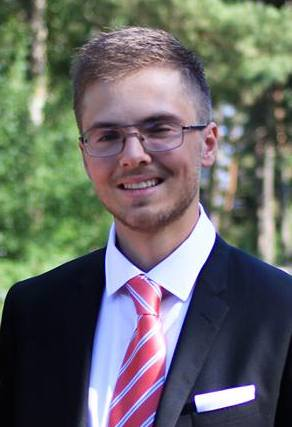
\includegraphics[width=0.13\linewidth]{stefan} & 
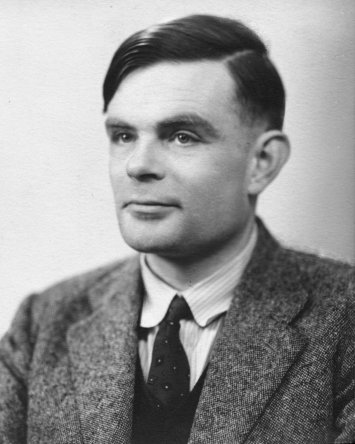
\includegraphics[width=0.13\linewidth]{Alan_Turing_photo}
\end{tabular}} 
% Normally there will not be any pictures but we want
% these so that we can connect faces to names in the course
% We also want birthdates so that we can tell people with the same
% name apart
\date{}

\pagestyle{fancy}
\setlength{\headheight}{15pt}
\fancyhf{}
\lhead{DD2380 ai14} % DO NOT REMOVE!!!!
\rhead{A.K. Dhaka, D. Vidas, S. Annell, U. Wara} %% UPDATE WITH YOUR NAMES

\begin{document}

\nocite{*}

\maketitle
\thispagestyle{fancy}

\begin{abstract}
Natural Language Generation (NLG) is a Natural Language Processing (NLP) task of
generating natural language. The problem is well known and well researched, but
the field is far from being fully explored. In this paper, we propose an idea of
building a text generator based on Hidden Markov Model (HMM). HMM allows us to
append words in a sentence that depend on a whole sequence until that point,
unlike other methods, such as n-gram, which use only a certain number of words
to predict the next one. HMM parameters are additionally optimized using
Genetic Algorithm (GA). This type of text generators may outperform simple ones
and match the performance of a more complex generators.
\end{abstract}



\clearpage

%%%%%%%%%%%%%%%%%%%%%%%%%%%%%%%%%%%%%%%%%%%%%%%%%%%%%%%%%%%%%
%%%%%%%%%%%%%%%%%%%%%%%%%%%%%%%%%%%%%%%%%%%%%%%%%%%%%%%%%%%%%
\section{Introduction}
\label{sec:intro}
Natural Language Generation(NLG) is the field of generating natural language for
a computer from a knowledge base or some information that the system can
understand. Some fields where the NLG is beeing applied are weather
forecast generation, summarize statistical data extracted from a database and
describing chains of reasoning performed by a system~\cite{nlgsystem01}.

This paper is about designing, implementing and comparing different methods of
generating news based on topic headlines that are given as an input to the
system. The news should be a few sentences long and be relevant to the topic,
not necessarily correct information but still relevant. The knowledge base is
going to be built up from news articles that in some way teaches our system.
Which means that Natural Language Processing (NLP) needs to be implemented for
building the database and tagging / structuring the words, allowing our system
to form sentences that are meaningful and semantically as correct as possible.

This is very interesting field of research and a good topic to study because it
incorporates several complicated tasks that are useful in wide variety of
applications. First of all, it is very difficult for a computer to understand
the content of a text, there has been a lot of work done in this field and we
will apply one of few different methods for this. It is also hard for a computer
to construct sentences that are correct semantically because of the
complexity of a natural languages, such as English as mentioned in
\cite{nlgScratch}. This fact raises another problem, which is the infinite
number of combinations of words. Furthermore, the aggravating circumstance that
the language (both dictionary and the grammar) is continuously evolving, makes
it even harder to define a specific set of rules that apply all the time,
considering that our datasets (news) are written by numerous authors and in
different time instants. NLG systems broadly have three subcomponents:text
planning, sentence planning and surface realisation.
In text planning, content and target of the text are detremined, During sentence
planning, syntactic and lexical means are ascertained whereas in realisation, 
actual words are strung together to give form to the basic structure which comes out
of sentence planning. 
It is also preferred if the results are benchmarked in some systematical way,
either manually (which is not preferred), semi-manually where the system might
give suggestions and the operator help the computer or it is done completely
automated (which is also quite hard).


\subsection{Contribution}
It is very hard for a computer to communicate with a human since the language is
very complex and it is hard to replicate and the language is one of the big
borders between computers and humans which makes this field of research very
interesting. The method that we are presenting is a new and interesting way to
generate text focused on a topic using Hidden Markov Models (HMM) and genetic
algorithm.

\subsection{Outline}
In Section~\ref{sec:relwork} previous work is recognized and the papers we have
researched to support our work is presented. Section~\ref{sec:method} contains
an overview on how we are going to solve the problem, and why we are choosing a
specific method and also how we are implementing the system. The result of the
implementation is presented in Section~\ref{sec:exps} and the whole paper is
summarized and concluded in Section~\ref{sec:summary}.

%%%%%%%%%%%%%%%%%%%%%%%%%%%%%%%%%%%%%%%%%%%%%%%%%%%%%%%%%%%%%
%%%%%%%%%%%%%%%%%%%%%%%%%%%%%%%%%%%%%%%%%%%%%%%%%%%%%%%%%%%%%
\section{Related work}
\label{sec:relwork}

The field of NLG and NLP are two very large fields that are subfields of
artificial intelligence and computational linguistics. A lot of research has
been done in these fields, although the fields are far from fully explored. Some
of the earliest work in this field was performed in the 1970's by people like
Goldman and Davey, where they helped to define the main problems in NLG 
as explained in \cite[p.~19-20]{buildingNLG}, where they also mention that NLG
started to be researched allot during 1980's by people like McKeown and Appelt
that had a big impact on how the subsequent research was going to be performed on NLG.
The field had a big increase in the 1990's where allot of real-world applications were made,
like the weather forecast system FOG.

The paper Building Applied Natural Language Generation
Systems~\cite{nlgsystem01} is about the architecture and how to structure your
NLG system when designing it. They describe six main tasks that needs to be
performed when generating a text; content determination, discourse planning,
sentence aggregation, lexicalization, referring expression generation and
linguistic realisation. They also discuss the sub components the system
needs to design and the algorithms, using which the different subproblems can be
solved. The main use of this paper is the structure of the generation part of
the system, but also suggestions and pointers on how the arising problems can be
solved.

Usage of HMMs in text generation is mentioned in~\cite{hmmnlg} where the model
is used in a task-oriented environment. Authors describe HMM generation process
to be very similar to POS (part of speech) tagging. States represent words, and
state sequences, word phrases. The model is designed from the corpus data
using ABL algorithm and it learns using the Baum-Welch algorithm.

These papers  ~\cite{poseval} ~\cite{bleueval} researched some different methods for evaluating Natural Language Generation systems, by comparing automated methods and human evaluation methods. Where  ~\cite{bleueval} propose methods like Bleu, NIST and Rogue which looks at the words of the generated sentence, and compares it to a reference. ~\cite{poseval} Suggests a pos tagging method, that breaks up the sentences into POS tags, and compares it to a big reference corpus.
They both discuss the pros and cons of the evaluation systems and suggests that a combination of automated methods should be used, since the different automated methods covers different parts of the text.

%%%%%%%%%%%%%%%%%%%%%%%%%%%%%%%%%%%%%%%%%%%%%%%%%%%%%%%%%%%%%
%%%%%%%%%%%%%%%%%%%%%%%%%%%%%%%%%%%%%%%%%%%%%%%%%%%%%%%%%%%%%
\section{My method}
\label{sec:method}

\subsection{Hidden Markov Models}

An n-gram models have been used for the task of NLG~\cite{nlgngram}. n-gram models use the
statistical property of co-occurrances to calculate the most likely word to
appear given previous (n-1) grams. Intuition would tell us that a higher n gram
model will perform better than a lower one as the samples will be fewer and are
more likely to be semantically correct but will be much more computationally
intensive. But there are  also some problems with n-gram models. They perform
the task of surface-realisation without having to need any grammar or knowledge
of semantics. Also in case where there are several sentences and the idea has to
flow with the sentences, they will perform poorly. Our objective is to give
better performance than a generator using a trigram.

This task mainly contains two parts: determining what to say and how to say.
The information decision (what to say) part can be done by using a statistical
method on the training set to determine the most commonly occurring noun words
with the given keywords. For example a keyword like "INDIA" can have
"population", "Gandhi", "Himalayas", "poor" as the set of possible information
generation candidates.

We propose to use HMMs for the surface generalisation task (how to say). HMMs
have been used with very good results in the fields of speech recognition and
also in NLU (Natural Language Understanding)~\cite{hmmsr}. The idea of HMM in this work is to
do something like the inverse of what POS Tagging does. In POS Tagging, an input
string of words is mapped to a hidden sequence of semantic POS tags. Here, the
sequence of POS tags can be determined by training it with data from various
news articles like Guardian, BBC, CNN. The POS Tags then can serve as the
observations in the HMM model and the words as the hidden states.  With the
different candidates for information, they can be trained by a HMM model and
then evaluated by a function which will select the best candidate out of them.
With the different candidates for information, they can be trained by a HMM
model and then evaluated by a function which will select the best candidate
out of them.

We also think to train the model parameters by a genetic algorithm to introduce
more randomness and to avoid problems of local minima.
To have more variation we intend to use WORDNET, so we can have multiple ways of
generating sentences, all having the same meaning.


\subsection {Performance measures for experiments}

As in other scientific fields, it is crucial to test how well our systems,
modules and algorithms work. This type of performance measure is called
evaluation. There are three techniques of evaluating NLG systems: task-based,
human ratings and metrics~\cite{evalnlg}. In our project we are going to use
human ratings and metric evaluations.

Evaluation gives as an output the ``goodness'' of a sentence or a text. The
``goodness'' is defined by three characteristics: fluency, adequateness and
readability~\cite{evalmethods}. It is often a difficult task to assess each
characteristic.
Human ratings are based on opinions of individuals rating the given the given
text. These types of evaluations are subjective and hard to measure. But the
main advantage is the that the natural language is made for interactions between
people and we can evaluate texts more accurately than machines. In our project
we will spend a certain amount of time evaluating our models ourselves and with
the help of others to reduce the bias.

Metric evaluations are based on software evaluations of generated text. They are
more objective than human ratings, but also less reliable. Most evaluators
compare generated text with texts written by people to compute the score. In our
project, we are going to use one or more of the following metric evaluators:
BLEU, NIST, METEOR; which ever proves to be most reliable~\cite{autoeval}.

\subsection {Measure success of the project work or approach}

The main task of the project is to successfully implement HMM text generator.
Besides HMM text generator, we are also going to implement simple n-gram
generators such as bigram and trigram. To measure success of the project
approach, we are going to use performance measures listed above, as well as
comparison between HMM and n-gram generator. If our hypothesis proves to be
true, HMM will perform better than bigram and trigram.
\subsection {Measure the progress during the course of\\ the project}

The project is divided into several stages. In the beginning, we will set the
hypothesis and elaborate details regarding the same. By analyzing collected
research papers, we will make decisions regarding implementation details,
improvements and alterations, and also define performance expectations of our
approach.

Second stage is the implementation. During this stage, we will implement bigram,
trigram and HMM text generators (and genetic algorithm for HMM optimization if
needed). In the same time we will also test our application to ensure algorithm
correctness.

Finally, we will run experiments (evaluations) mentioned above and alter
parameters accordingly to achieve better results.

During the course of the project, we will record our progress based on the
project plan described above. Prediction of the time consumption will be made
for each of the stages. Using those predictions, we will adjust the pace of the
project progress for the purpose of completing the task in time.

\subsection{Implementation}
\label{sec:impl}

Implementation will be done shortly.

%%%%%%%%%%%%%%%%%%%%%%%%%%%%%%%%%%%%%%%%%%%%%%%%%%%%%%%%%%%%%
%%%%%%%%%%%%%%%%%%%%%%%%%%%%%%%%%%%%%%%%%%%%%%%%%%%%%%%%%%%%%
\section{Experimental results}
\label{sec:exps}

The result of our experiments, will be written when we have done the implementation.


\subsection{Experiemntal setup}

The system design will be presented when the setup is done.

%%%%%%%%%%%%%%%%%%%%%%%%%%%%%%%%%%%%%%%%%%%%%%%%%%%%%%%%%%%%%
%%%%%%%%%%%%%%%%%%%%%%%%%%%%%%%%%%%%%%%%%%%%%%%%%%%%%%%%%%%%%
\section{Summary and Conclusions}
\label{sec:summary}
To be written later.


%%%%%%%%%%%%%%%%%%%%%%%%%%%%%%%%%%%%%%%%%%%%%%%%%%%%%%%%%%%%%
%%%%%%%%%%%%%%%%%%%%%%%%%%%%%%%%%%%%%%%%%%%%%%%%%%%%%%%%%%%%%
\bibliography{ref}
\bibliographystyle{plain}


\end{document}